\documentclass[11pt]{article}
\usepackage[utf8]{inputenc}
\usepackage[T1]{fontenc}
\usepackage{graphicx}
\usepackage{xcolor}
\usepackage{listings}
\usepackage{textcomp}
\usepackage[most]{tcolorbox}
\usepackage{pythonhighlight}
\usepackage{minted}
\usepackage{lscape}
\usepackage{rotating}
\usepackage{svg}
\usepackage[titletoc,title]{appendix}
\usepackage{animate}
\usepackage{subcaption}
%\usepackage{subfig;subfigure}
%\usepackage[dotinlabels]{titletoc}

%\usepackage[autostyle]{csquotes}

\usepackage[backend=bibtex,citestyle=authoryear,maxnames=1]{biblatex}
\addbibresource{biblio.bib}

\newcommand{\source}[1]{\vspace*{-0.4cm}\caption*{\textit{Source: {#1}}}}
\renewcommand{\contentsname}{Table of contents}
\newcommand{\mycite}[1]{ (\cite{#1})}
\newcommand{\comopa}{ (COMOP TVB 1 2010\nocite{comop-a})}
\newcommand{\comopb}{ (COMOP TVB 2 2010\nocite{comop-b})}
\newcommand{\millenium}{ (Millennium Ecosystem Assessment 2005\nocite{millenium})}
\newcommand{\tocheck}[1]{\textcolor{lightgrey}{#1}}
\newcommand{\tool}{\emph{FragScape}}
\newcommand{\qgis}{\emph{QGIS}}
\newcommand{\grass}{\emph{GRASS}}
\renewcommand{\refname}{Bibliographie}
\newcommand{\myfigureref}[1]{Figure \ref{#1} : \hyperref[#1]{\nameref{#1}}\dotfill\pageref{#1}}
\newcommand{\meff}{effective mesh size}
\newcommand{\Meff}{Effective mesh size}



\lstset{upquote=true,
    language=Python,
    showspaces=false,
    basicstyle=\small\ttfamily,
    %numbers=left,
    %numberstyle=\tiny,
    commentstyle=\color{gray}
    xleftmargin=1cm,
    % Code design
    identifierstyle=\color{editorGray},
    keywordstyle=[1]\color{editorBlue}\bfseries,
    keywordstyle=[2]\color{editorBlue}\bfseries,
    keywordstyle=[3]\color{editorBlack}\bfseries,
    keywordstyle=[4]\color{editorBlue}\bfseries,
    commentstyle=\color{editorGray}\ttfamily,
    stringstyle=\color{editorGreen}}

\definecolor{FunctionName}{rgb}{0,150,0}

% 2079971ms

\definecolor{editorLightGray}{cmyk}{0.05, 0.05, 0.05, 0.1}
\definecolor{editorWhite}{cmyk}{0, 0, 0, 0}
\definecolor{editorOrange}{cmyk}{0, 0.8, 1, 0}
\definecolor{editorBlue}{cmyk}{1, 0.6, 0, 0}
\definecolor{editorGreen}{rgb}{0, 0.5, 0}
\definecolor{editorGray}{black}{0.9}

\input{defs}

\usepackage{lipsum}
\usepackage{arydshln}
\usepackage{hyperref}

\usepackage{biblatex}
\addbibresource{biblio.bib}

\usepackage{fancyhdr}
\usepackage{lastpage}

\usepackage{indentfirst}

\pagestyle{fancy}
\fancyhf{}

\setlength{\headsep}{1.3in}
\setlength{\voffset}{-30pt}
\setlength\parindent{0pt}


\let\tempone\itemize
\let\temptwo\enditemize
\renewenvironment{itemize}{\tempone\addtolength{\itemsep}{-0.5\baselineskip}}{\temptwo}
\renewenvironment{enumerate}{\tempone\addtolength{\itemsep}{-0.5\baselineskip}}{\temptwo}


%%%%%%%%%%%%%%%
% Title Page
\bigskip
%\title{Développement d'un plugin \emph{QGIS} pour modéliser les déplacements de la faune par la méthode de perméabilité des milieux pour la cartographie des continuités écologiques}
%\title{Titre quand meme plus court sinon c'est relou}
\bigskip

\date{\today}
%\summary{}
%%%%%%%%%%%%%%%

\begin{document}

\renewcommand{\appendixtocname}{Annexes}
\renewcommand{\appendixpagename}{\color{color1}{Annexes}} 
\sloppy

%\pagestyle{style2}

\vspace{4cm}

\maketitle

\clearpage

\pagestyle{style1}

\setlength{\headsep}{0.9in}

\tableofcontents

\hspace{4cm}

%\section*{Table des figures}


%\myfigureref{biogeoFragm}


%\pagebreak

%\section*{Table des figures}

\pagebreak

\section{Overview}

\tool\ is a \qgis\ plugin that computes landscape fragmentation metrics defined in paper "Landscape division, splitting index, and effective mesh size: new measures of landscape fragmentation" \mycite{jaeger}.
Among these metrics, \meff\ has been widely used to quantify landscape fragmentation. \tool\ defines a 4 steps process from raw data to computed metrics and allow user to save configuration so that results can be reproduced with same context.

\subsection{Landscape fragmentation metrics}
\label{sec:metrics}

Jaeger defined in his paper\mycite{jaeger} three new measures of landscape fragmentation:
\begin{itemize}
    \item landscape division
    \item splitting index
    \item effective mesh size
\end{itemize}

To compute these measures, landscape elements assessed as fragmenting are removed. Remaining areas are called patches. Landscape is then composed of $n$ patches. A patch area is denoted by $A_i$ with $1 \leq i \leq n$. The total area of the region is denoted by $A_t$.

\subsubsection{Landscape division}

The degree of coherence ($C$ or $COH$), an auxiliary measure, is defined as the probability that two points chosen randomly in a region are connected (e.g. not separated by fragmentation elements such as roads or urban areas):

The degree of landscape division ($D$ or $DIVI$) is defined as the probability that two points chosen randomly in a region are $not$ connected:

\hspace*{-0.5cm}
\begin{minipage}[c][1cm]{.46\linewidth}
\begin{align*}
C = \sum_{i=1}^{n}(\frac{A_{i}}{A_{t}})^{²}
\end{align*}
\end{minipage}
\begin{minipage}[c][1cm]{.46\linewidth}
\begin{align*}
D = 1 - C
\end{align*}
\end{minipage}

\subsubsection{Splitting index}

The  splitting index ($S$ or $SPLI$) is defined as the number of patches one gets when dividing the total region into parts of equal size (meshes) in such a way that this new configuration leads to the same degree of fragmentation of initial configuration:
\begin{align*}
S = \frac{A_{t}^{2}}{\sum_{i=1}^{n}A_{i}^{2}}
\end{align*}

It can be interpreted as the effective mesh number of a grid with a constant mesh size dividing the region into S patches which all have the size $A_{t} / S$.

\subsubsection{Effective mesh size}

The effective mesh size ($m$ or $MSIZ$) denotes the size of the areas when the region is divided into $S$ areas (each of the same size $At/S$) with the same degree of landscape division as for the initial configuration:
\begin{align*}
m = \frac{A_{t}}{S} = \frac{1}{A_{t}}\sum_{i=1}^{n}A_{i}^{2}
\end{align*}

Splitting density ($s$ or $SDEN$) is defined as the number of meshes per unit area.
Net product ($N$ or $NPRO$) is defined as the product of the effective mesh size and the total area of the region:

\hspace*{-0.5cm}
\begin{minipage}[c][1cm]{.46\linewidth}
\begin{align*}
s = \frac{S}{A_{t}} = \frac{A_{t}}{\sum_{i=1}^{n}A_{i}^{2}} = \frac{1}{m}
\end{align*}
\end{minipage}
\begin{minipage}[c][1cm]{.46\linewidth}
\begin{align*}
N = m.{A_{t}} = \sum_{i=1}^{n}A_{i}^{2}
\end{align*}
\end{minipage}


\subsubsection{Cross-Boundary Connection (CBC) method}
\label{sec:cbc}

As other patch-based landscape metrics, above metrics can be biased by the boundaries and the extent of a reporting unit if the boundaries fragment patches. This issue is called the "boundary problem" and has been addressed  in paper "Modification of the effective mesh size for measuring landscape fragmentation to solve the boundary problem"\mycite{moser}.

New method called \textit{cross-boundary connections} (CBC) includes area outside boundaries. The complete area of a patch, regardless of boundaries, is denoted by $A_{i}^{cmpl}$. The formula of effective mesh size according to CBC method ($m_{CBC}$ or $CBC\_MSIZ$) is:
\begin{align*}
m_{CBC} = \frac{1}{A_{t}}\sum_{i=1}^{n}A_{i}.A_{i}^{cmpl}
\end{align*}

\frameboxbegin{Métriques CBC}
\textbf{\color{red}In CBC mode, only 2 metrics are defined : effective mesh size and net product}
\frameboxend

\bigskip

\subsection{Computation methods}
\label{sec:mode}

Metrics are computed from a layer of natural areas patches.

\tool\ is designed to include patch layer creation from raw data (land cover, roads, ...) following a step-by-step procedure (cf section \ref{sec:steps}): natural areas selection from land cover and integration of additional data.

There are 2 computation methods depending on input data format, extent, precision needs and available computing resources. Vector mode is appropriate for vector land cover in case the amount of data is reasonable (cf section \ref{sec:execTime}). Raster mode is appropriate otherwise (raster land cover, large extent, high geometric precision, ...). 

\subsubsection{Vector mode}

In vector mode, features are selected from land cover layer and dissolved (one feature of type MultiPolygon).

It is then possible to integrate additional data such as roads network, hydrographic network, or any missing data in initial layer. For each data source, features can be selected (paved roads for instance) and a buffer can be applied to modelize footprint for linear data. These selections are then merged with land cover, by union or difference depending on their contribution to fragmentation or to natural areas. Resulting layer is then dissolved and casted to single geometry (Polygon) to finally get a correct patch layer for metrics computation.

\subsubsection{Raster mode}

In raster mode, input data can be vector or raster but output layers are in raster format anycase (rasterization and reprojection according to extent and resolution parameters).

Resolution value is very important because it defines computation precision but also random-access memory (RAM) needed. If land cover is already in raster format, resolution shall be the same than land cover layer.

Land cover layer is reclassified: 1 for natural areas (selected classes), 0 for fragmentation data (unchecked classes).
Additional data is reprojected and classified same way. Resulting layers are then merged according to specified ranking order in graphical user interface.

\subsection{Installation}

\tool\ is a \qgis\ plugin. \tool\ is  cross-platform: tests have been performed on Ubuntu bionic, Windows 10 and macOS Sierra.

\frameboxbegin{Prerequisites}
\textbf{\color{red}\qgis\ version must be superior to 3.4.0.}

\begin{itemize}
    \item \textbf{\color{red}\qgis\ version must be superior to 3.4.0.}
    \item \textbf{\color{red}Python libraries \emph{scipy} et \emph{numpy} must be already installed to use raster mode (cf section \ref{sec:err}).}
\end{itemize}
\frameboxend

To install \tool, open \qgis:
\begin{enumerate}
    \item go to \texttt{Extension} menu
    \item open \texttt{Install/Manage extensions} dialog
    \item go to \texttt{Parameters} tab and check that \texttt{Show experimental plugins} option is checked 
    \item go back to \texttt{All} tab, search for \tool, select it and click on \texttt{Install plugin} button
\end{enumerate}

Once installed, \tool\ icon \includesvg{pictures/vector_grid.svg} shall appear in tools panel.

If not, go to \texttt{Extension} menu and a \tool\ entry shall be present.

If not, installation failed. Please check error message or contact support team.

\bigskip

\subsection{Graphical User Interface (GUI) overview}

Figure \ref{fig:paramsTab} show an overview of \tool\ GUI. It contains 4 main components :
\begin{itemize}
    \item top icons bar : action icons (configuration management, language switch)
    \item right panel : description of current step
    \item bottom progress bar : shows progress of current process
    \item main frame : current step content
\end{itemize}

In main frame, current step can be composed of :
\begin{itemize}
    \item parameters that must be set (such as \texttt{Workspace})
    \item visualisation table that displays current configuration/results
    \item action buttons (such as \texttt{Launch selection})
\end{itemize}

\begin{figure}[h!]
    \centering
    \includegraphics[scale=0.7]{pictures/paramsTabEn_v2.png}
    \caption{\tool\ v2.0 Graphical User Interface}
    \label{fig:paramsTab}
    %\source{\tool\ v1.0}
\end{figure}

\pagebreak

\section{Steps}
\label{sec:steps}

\tool\ defines a 4 step procedure from raw data to computed metrics.

\subsection{Parameters}

First step is to define global parameters used for current \tool\ project.

\texttt{Workspace} must be set before any processing as it defines \tool\ outputs path. Output file of each step is stored in \textit{Workspace/outputs}. Be careful when setting workspace as existing file can be overriden.

\texttt{Mode} defines processing chain executed to compute metrics (cf section \ref{sec:mode}). In raster mode, \texttt{Resolution} must be set to define pixel size in georeferenced unit (meter for a metric projection).

\texttt{Extent layer} defines data extent: data are clipped at layer limits. Optional in vector mode. In CBC mode, data extent must be larger than study area.

\texttt{Projection} is a projected coordinate reference system that must be set according to data geographic extent. It defines entities shape and area.

If option \texttt{Save intermediate layers} is checked, intermediate layers are stored in \textit{Workspace/tmp}. Otherwise, they are stored in \qgis\ \textit{processing} temporary directory (path is displayed in log when a layer is created).


\pagebreak

\subsection{Land cover}

Second step is to select target features from land cover layer. To do so:

\begin{enumerate}
    \item Select land cover layer (\texttt{Input layer} parameter).
    \item Choose \texttt{Mode} and \texttt{Selection field} in input layer is vector
    \item Press button \texttt{Show field values}
    \item Check land cover classes matching natural areas in \texttt{toSelect} column of table
    \item Press button \texttt{Launch selection}. Output layer is loaded in \qgis\ and saved in $Workspace/outputs$ ($landuseSelectionDissolve.gpkg$ in vector mode, $landuseSelectionWarp.tif$ in raster mode).
\end{enumerate}

\vspace*{-0.5cm}
\frameboxbegin{Selection mode}
There are 2 selections modes in In \texttt{Vector} mode:
\vspace*{-0.2cm}
\begin{itemize}
\item \texttt{By field values} to extract unique values from \texttt{Selection field}
\item \texttt{By expression} to extract features verifying specified expression (all features if expression is empty)
\end{itemize}
\vspace*{-0.2cm}
In \texttt{Raster} mode, unique values are extracted from first band.
\frameboxend

Figure \ref{fig:landuseTab} shows an example of land cover selection interface.

\begin{figure}[h!]
    \centering
    \includegraphics[scale=0.6]{pictures/landuseTabEn_v2.png}
    \caption{\tool\ v2.0 \textit{Land cover} tab}
    \label{fig:landuseTab}
    %\source{\tool\ v1.0}
\end{figure}

\subsection{Additional data}

Third step is to integrate additional data that would be missing in land cover. For instance: roads, river courses, wildlife crossing, ...

For each data source, user should:
\begin{enumerate}
    \item Select \texttt{Input layer}
    \item (optional) Filter input features according to specified \texttt{Expression} (all features if expression is empty).  Expression can be built with \includesvg{pictures/mIconExpression.svg} widget.
    \item Specify \texttt{Buffer} expression for line and point data in vector mode to modelize footprint. Expression must be a number and can be built with \includesvg{pictures/mIconExpression.svg} widget.
    \item Specify an \texttt{Identifier} (unique in project) for current selection
    \item Press \texttt{Save selection} button. Specified selection appears as a new line in visualisation table.
\end{enumerate}

Once all data selections saved, user should rank lines (for instance wildlife corridors on top of roads) and then press \texttt{Integrate additional data} button.

For each line, data is selected, buffer is applied (if defined) and layer is rasterized in raster mode. Output layers are then merged and integrated to result of previous step.

Final layer is loaded in QGIS and stored and savec in output directory ($landuseFragmSingleGeom.gpkg$ in vector mode, $landuseFragm.tif$ in raster mode).

\bigskip

\begin{figure}[h!]
    \centering
    \includegraphics[scale=0.6]{pictures/fragmTabEn_v2.png}
    \caption{\tool\ v2.0 \textit{Additional data tab}}
    \label{fig:fragmTab}
    %\source{\tool\ v1.0}
\end{figure}

\pagebreak

\subsection{Results}

Fourth step is to compute fragmentation metrics. To do so:

\begin{itemize}
    \item Specify \texttt{Input layer} (result of setp 3 by default).
    \item Specify \texttt{Reporting layer}. Metrics are computed for each feature of reporting layer. To compute metrics for an entire region, specify a layer with a single feature.
    \item Check \texttt{Include CBC metrics} if needed (see section \ref{sec:cbc})
    \item Select \texttt{Unit of area} (from square meter to square kilometer)
    \item Specify \texttt{Output layer}. If not specified, a memory layer is created.
    \item Press \texttt{Compute metrics} button.
\end{itemize}

\begin{figure}[h!]
    \centering
    \includegraphics[scale=0.6]{pictures/resTabEn_v2.png}
    \caption{\tool\ v2.0 \textit{Results} tab}
    \label{fig:resultsTab}
    %\source{\tool\ v1.0}
\end{figure}


Figure \ref{fig:resultsTab} shows results step interface. Once metrics are computed, output layer is loaded in \qgis\ and global effective mesh size (on the whole territory) is displayed. Output layer contains an attribute for each metric defined in section \ref{sec:metrics} and new fields:
\begin{itemize}
    \item \texttt{patches}: number of patches
    \item \texttt{At}: area of the reporting unit
    \item \texttt{sum\_Ai}: intersection area of patches and reporting unit
    \item \texttt{layer/path}: temporary layer containing initial reporting unit
    \item \texttt{divisor} : divisor matching unit of area (for instance 100 for are unit)
\end{itemize}

\pagebreak

\section{Example}

This section illustrates \tool\ use case with provided sample data (subdirectory \href{https://github.com/MathieuChailloux/FragScape/tree/master/sample_data/EPCI_Clermontais_2012}{\texttt{sample\_data}} in \tool\ plugin directory).

\begin{figure}[h!]
\centering
   \begin{subfigure}[b]{.48\textwidth}
      \includegraphics[width=\textwidth]{pictures/landuseInput.png}
      %\includegraphics[width=\textwidth]{pictures/CBC/landuseInput.png}
      \caption{Input data}
   \end{subfigure}
   \begin{subfigure}[b]{.48\textwidth}
      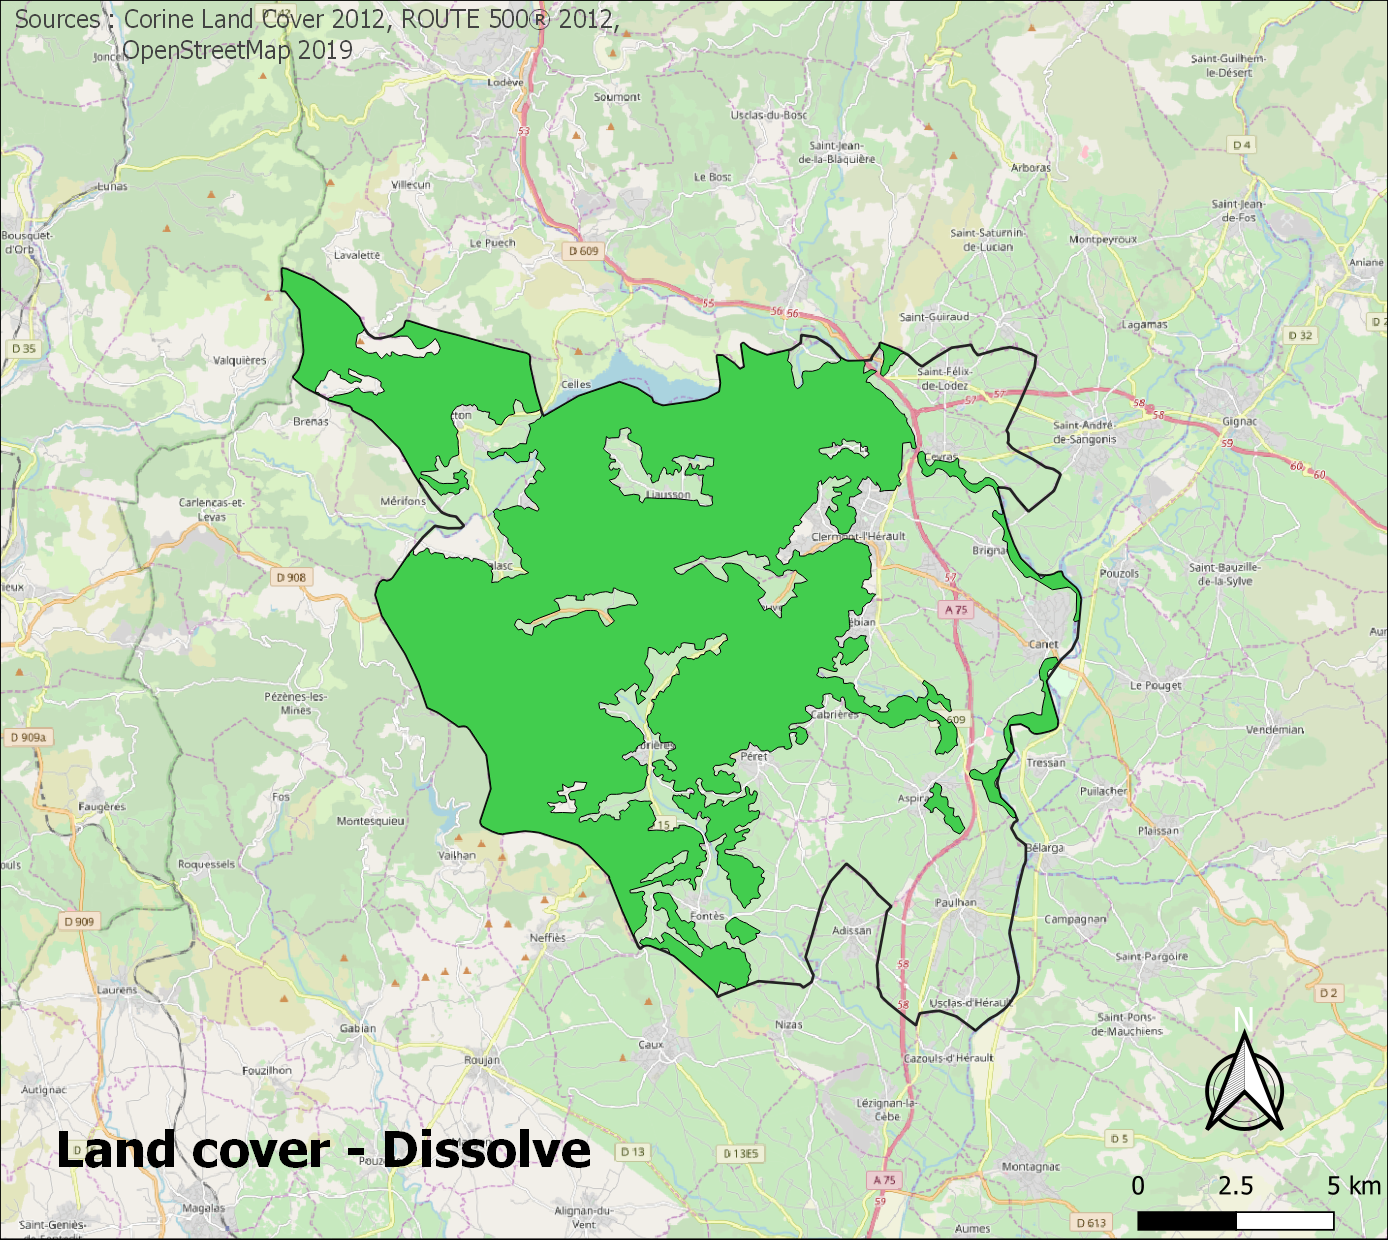
\includegraphics[width=\textwidth]{pictures/landuseDissolve.png}
      %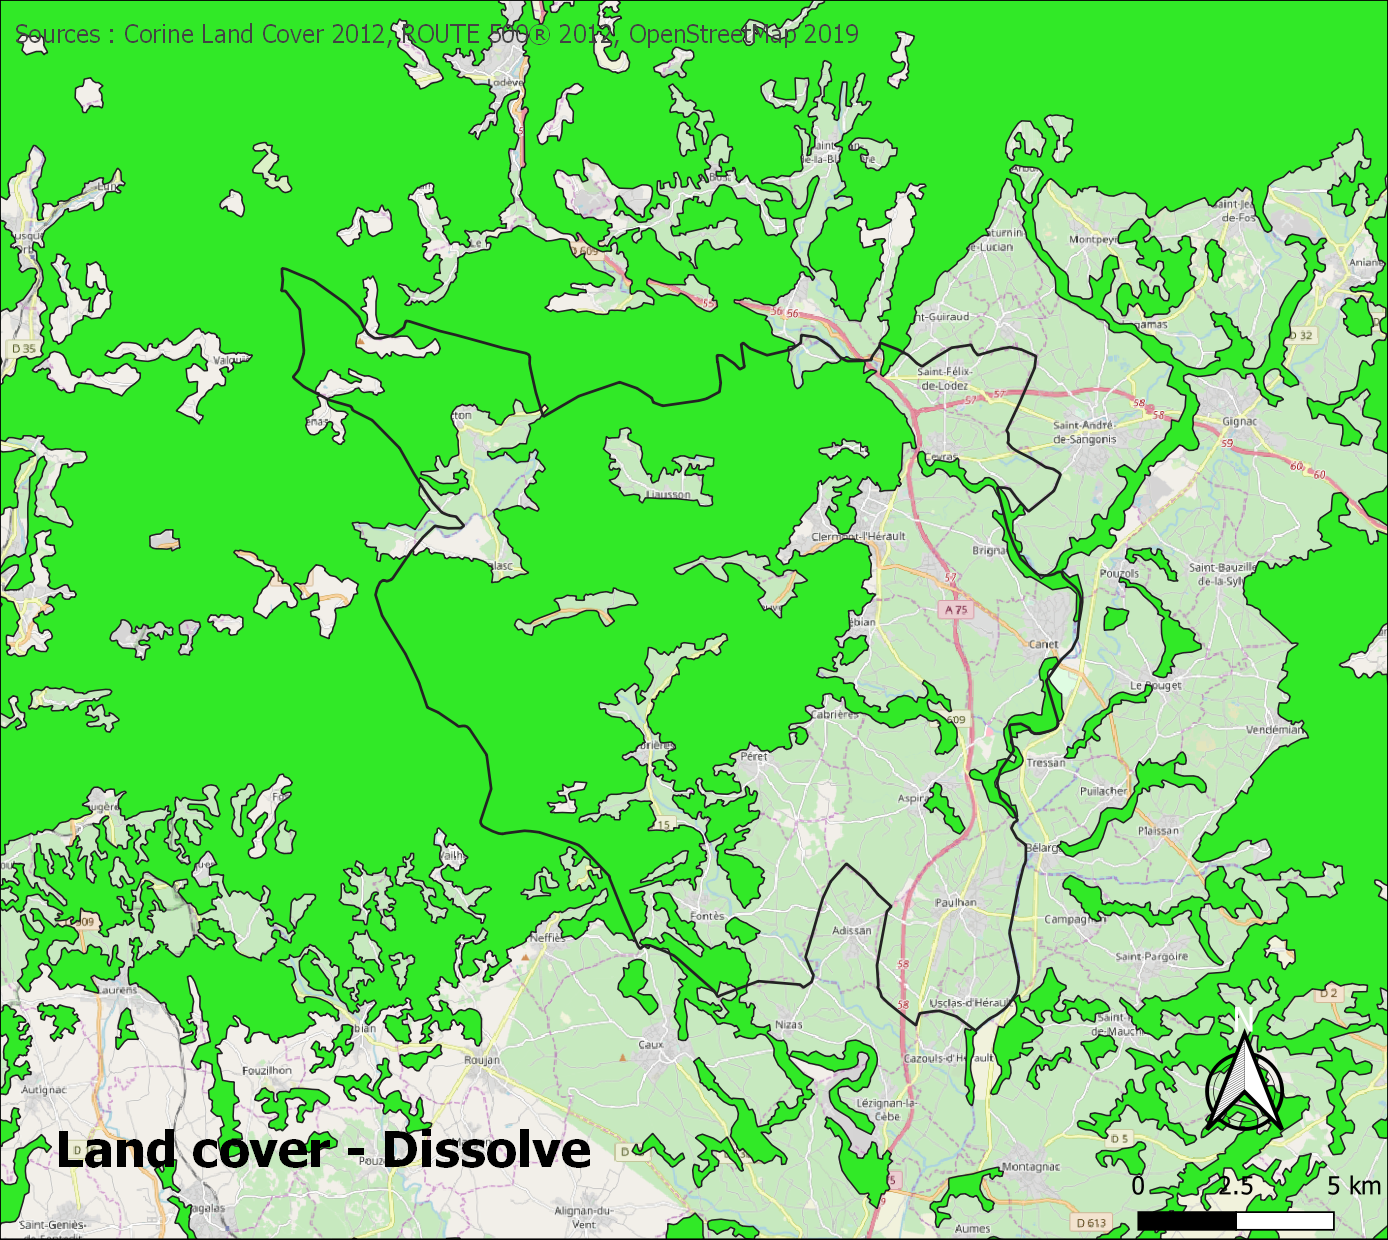
\includegraphics[width=\textwidth]{pictures/CBC/cbcLanduseDissolve.png}
      \caption{Step2}
   \end{subfigure}
   \begin{subfigure}[b]{.48\textwidth}
      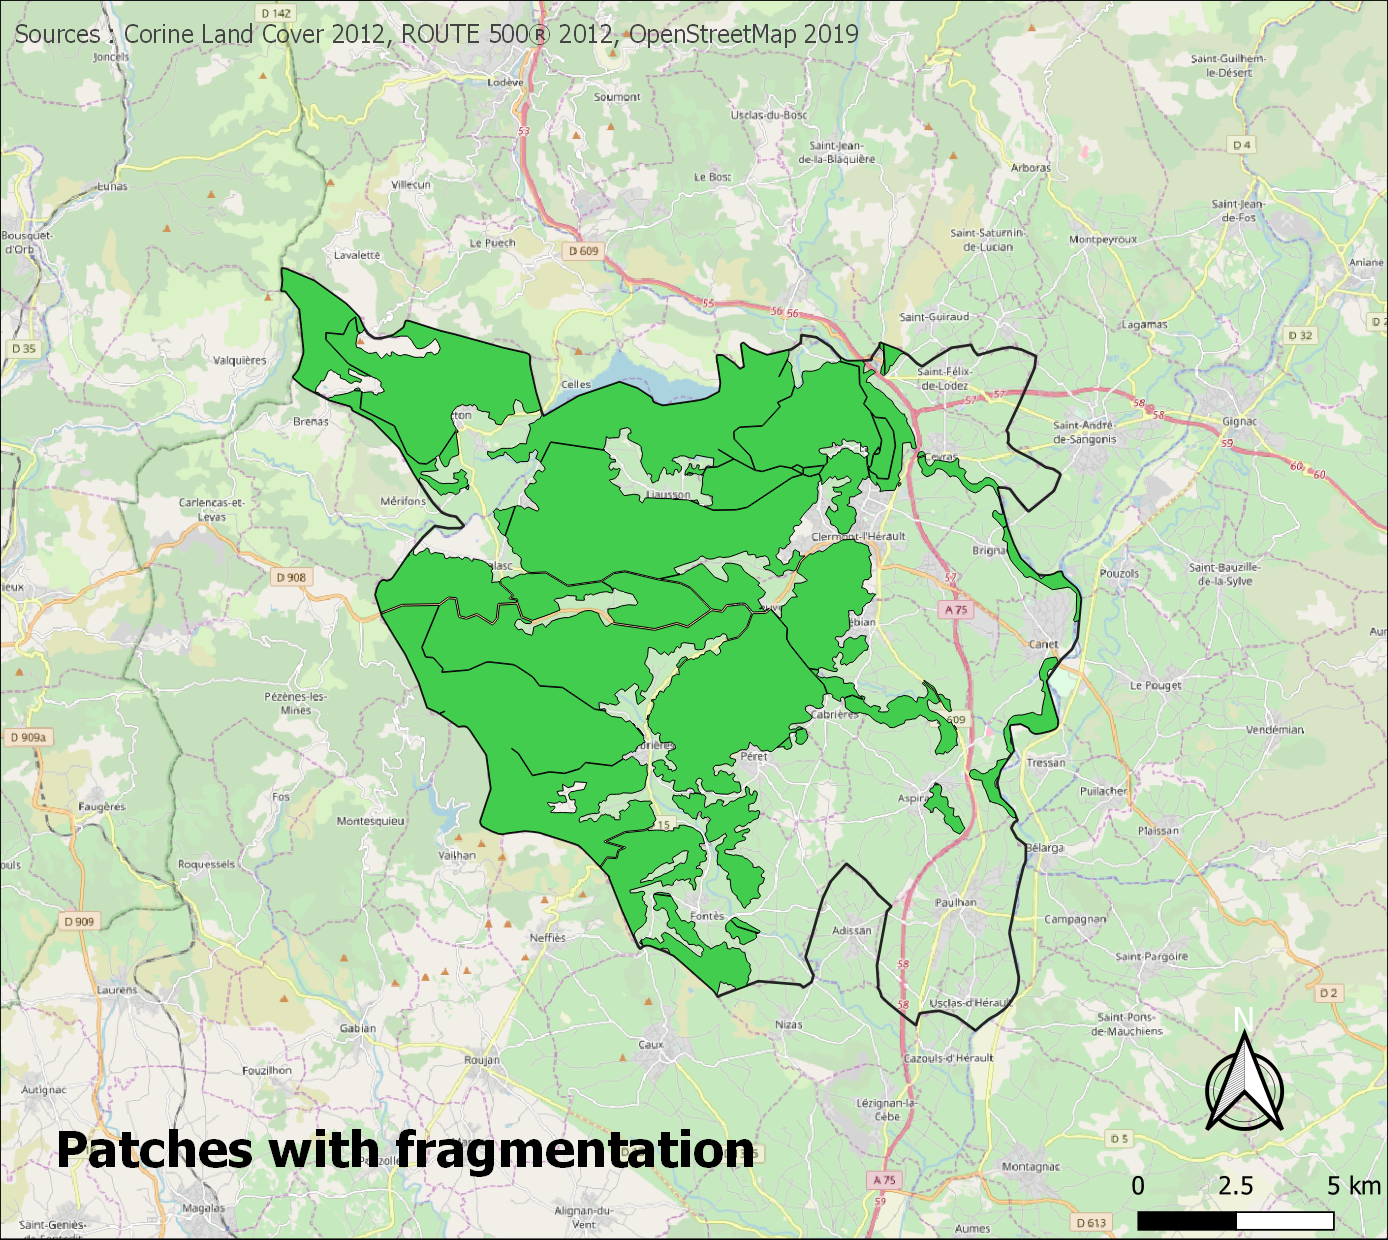
\includegraphics[width=\textwidth]{pictures/fragmPatches.png}
      %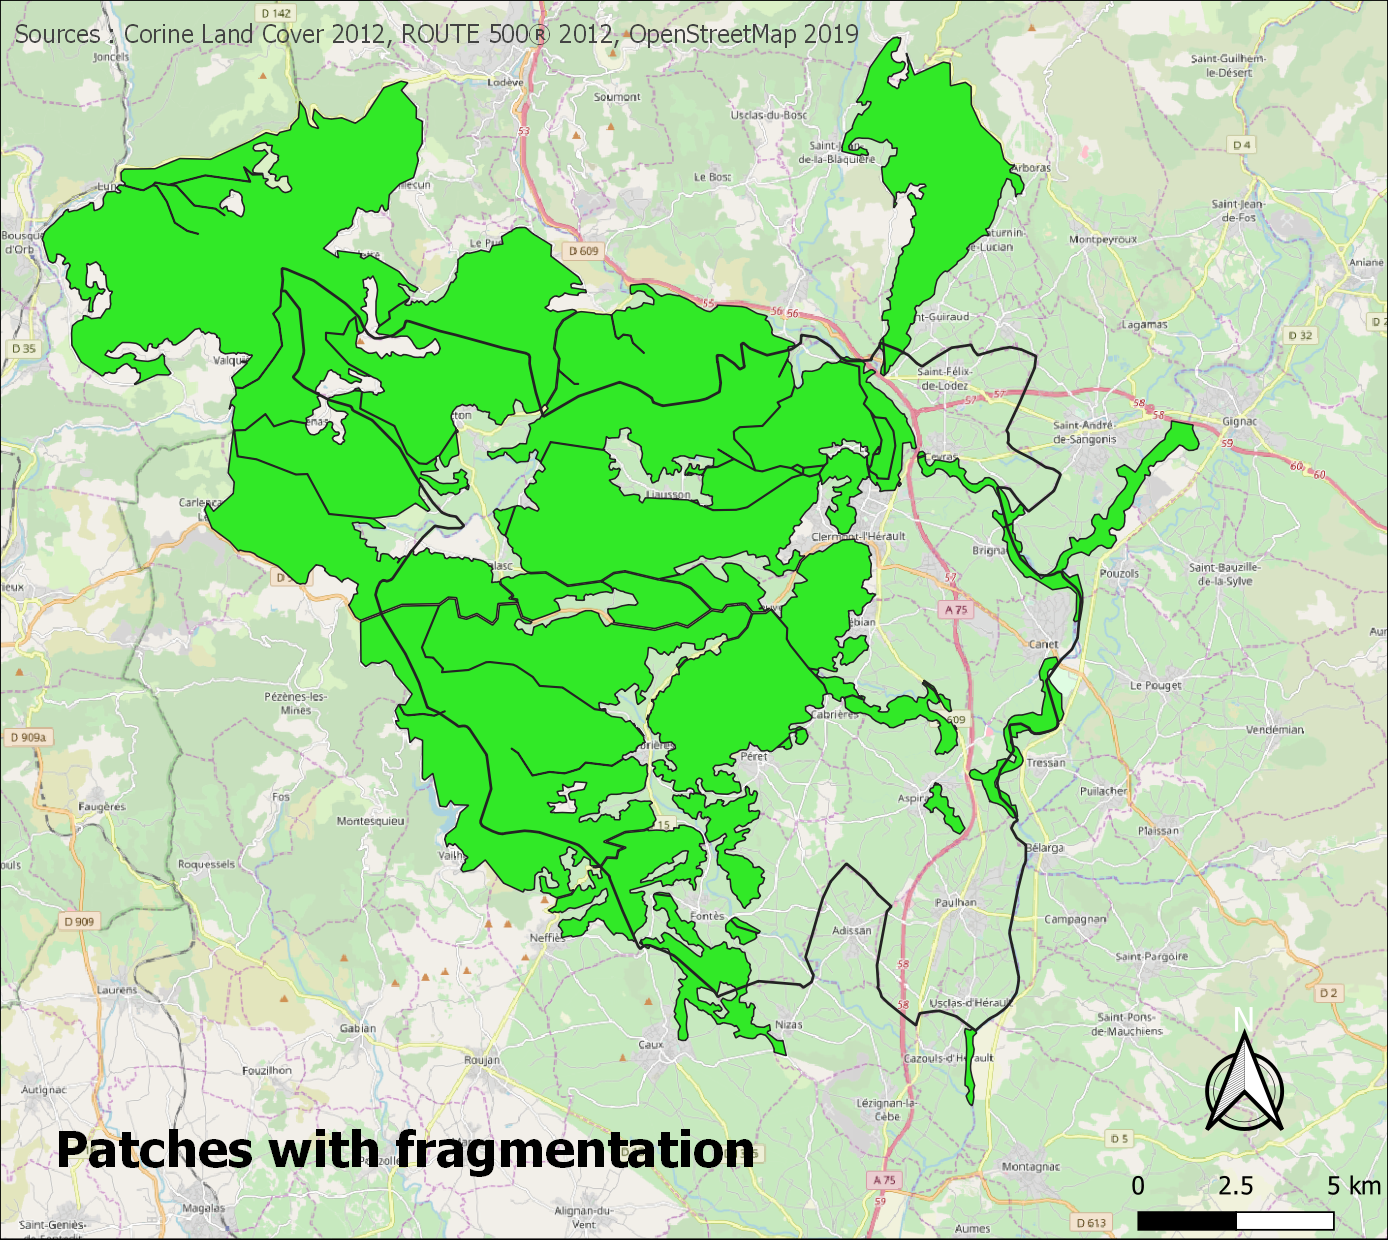
\includegraphics[width=\textwidth]{pictures/CBC/cbcFragmPatches.png}
      \caption{Step 3}
   \end{subfigure}
   \begin{subfigure}[b]{.48\textwidth}
      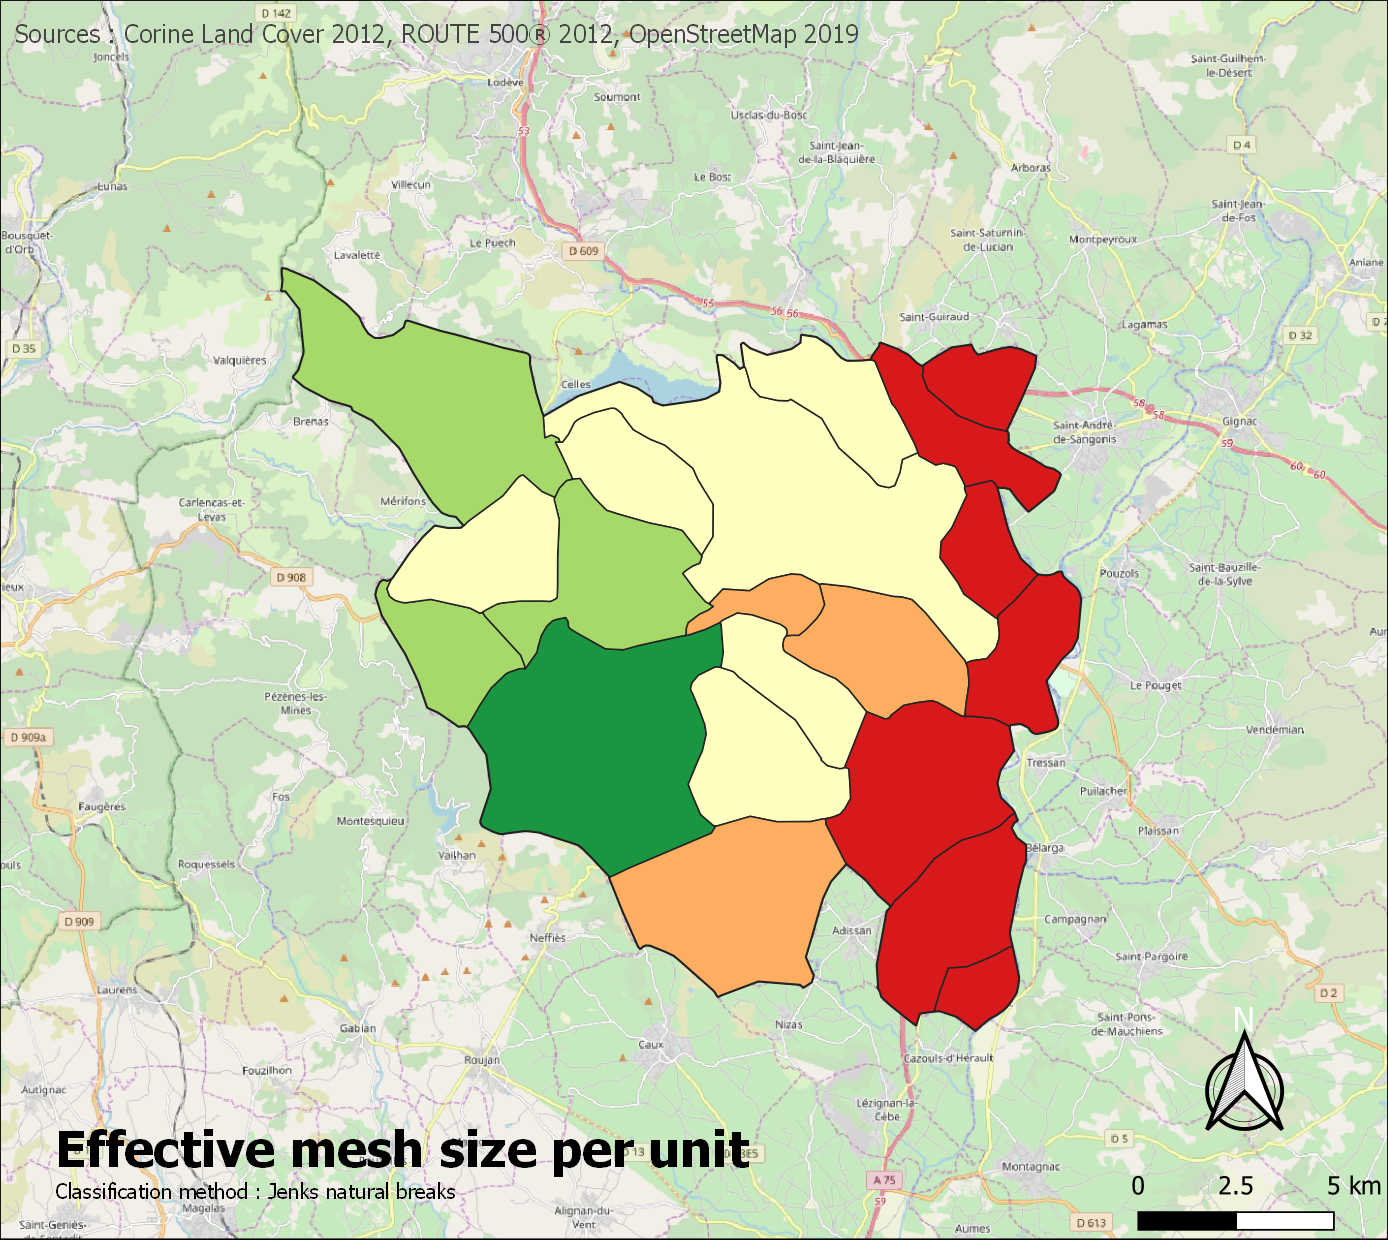
\includegraphics[width=\textwidth]{pictures/results.png}
      %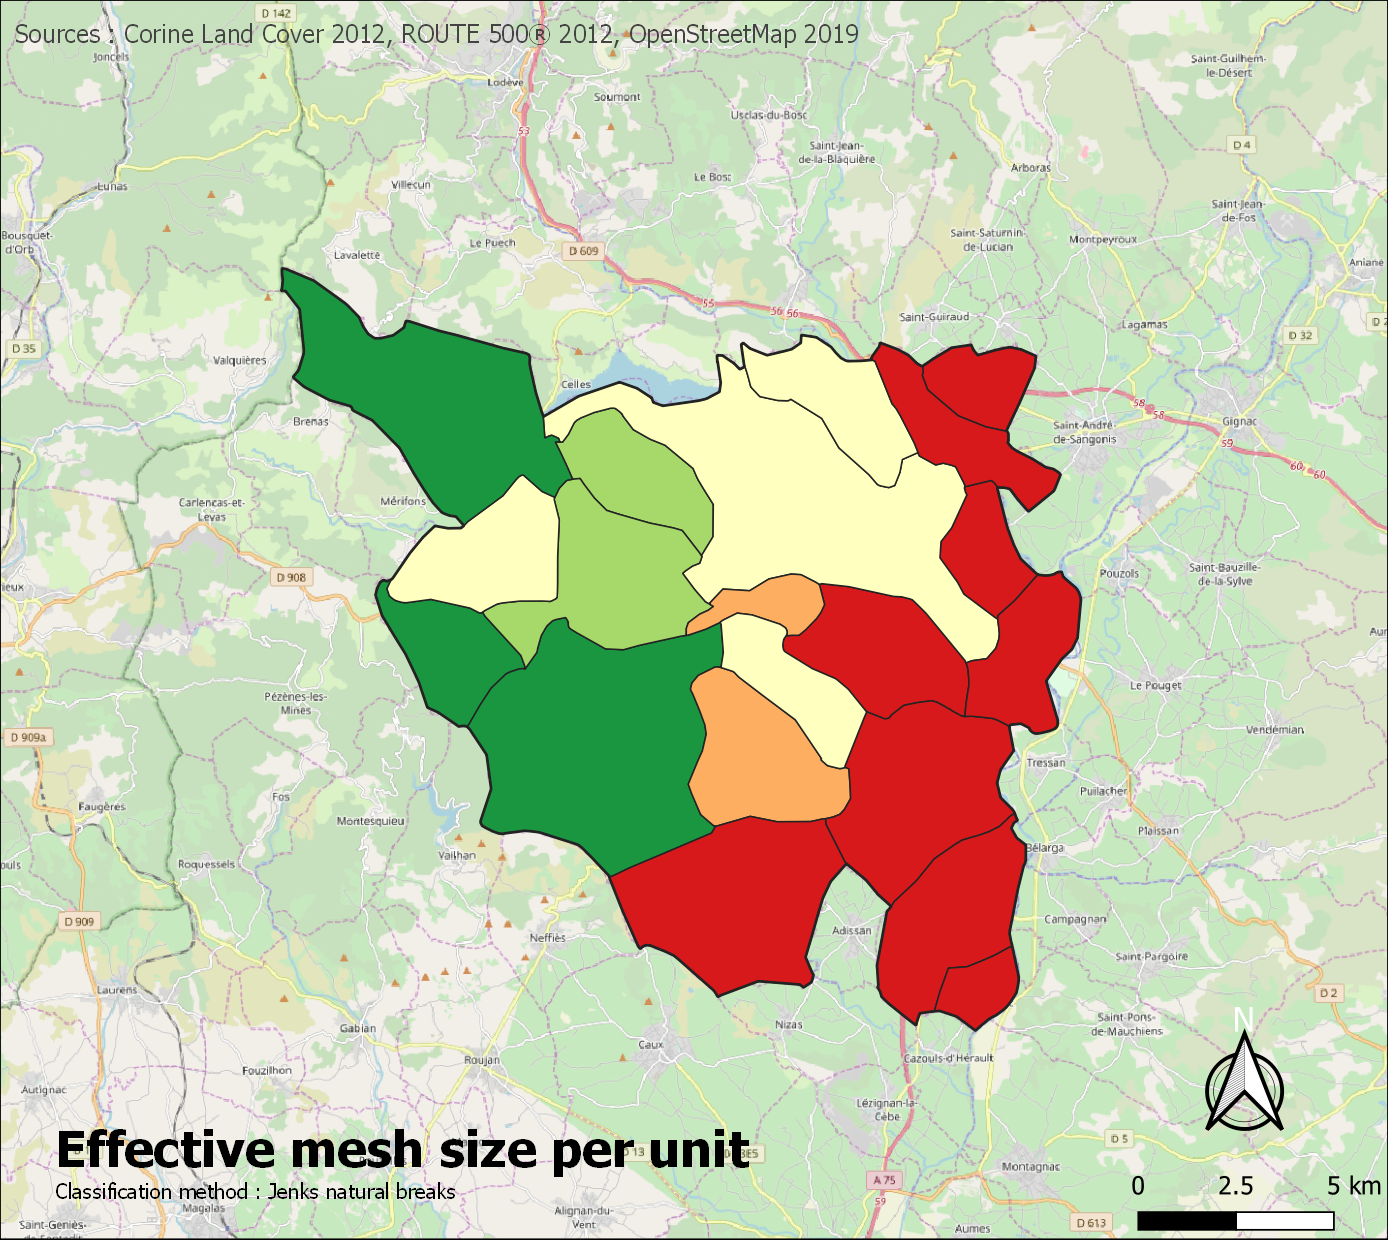
\includegraphics[width=\textwidth]{pictures/CBC/cbcResults.png}
      \caption{Step 4}
   \end{subfigure}
   \caption{\tool\ use case : from raw data to effective mesh size}
   \label{fig:usecase}
\end{figure}

Figure \ref{fig:usecase} shows input data and each step result.

To reproduce results:
\begin{itemize}
    \item Copy \texttt{sample\_data} to a local directory
    \item Open \tool
    \item Set workspace to \texttt{sample\_data/CUT}
    \item Open configuration file \texttt{EPCI\_Clermontais\_2012\_CUT.xml} from \ \includesvg[scale=0.6]{pictures/mActionFileOpen.svg} button
    \item Check that configuration has been correcty loaded
    \item Run steps 2 to 4
\end{itemize}

%Legends are not automatically generated.



%\animategraphics[autoplay,loop,width=\textwidth,controls,scale=0.5]{1}{pictures/Image_}{1}{4}

\section{To go further...}

\subsection{Execution time and memory}
\label{sec:execTime}

Use of \tool\ depends on available computing resource when applied to large territory with high level of geometric precision.

\subsubsection{Vector mode}

In vector mode, execution time can be very long depending on study area extent and geometric precision. Given execution times are \textbf{indicative values}.

Figure \ref{fig:benchCLC} show the evolution of execution time according to region extent (small region, big region, country) from \emph{Corine Land Cover} (vector data):


\begin{figure}[h!]
\begin{center}
\begin{tabular}{|c|ccc|}
    \hline
    Study area & Step 2 & Step 3 & Step 4\\
    \hline
    Hérault & <1mn & 1mn & 1mn \\
    Occitanie & 5mn & 11mn & 2mn \\
    France & 122h & 19h & 5h \\
    \hline
\end{tabular}
\end{center}
\vspace*{-0.5cm}
\caption{Execution time by extent}
\label{fig:benchCLC}
\end{figure}

Figure \ref{fig:benchOS} show the execution time according to data source geometric precision (\emph{Corine Land Cover} vs \emph{OCcupation du Sol Grande Échelle}) on a same territory (Hérault):

\begin{figure}[h!]
\begin{center}
\begin{tabular}{|c|ccc|}
    \hline
    Cas de test & Étape 2 & Étape 3 & Étape 4\\
    \hline
    CLC & <1mn & 1mn & 1mn \\
    OCSGE & 6h & 35h & 3mn \\
    \hline
\end{tabular}
\end{center}
\vspace*{-0.5cm}
\caption{Temps d'exécution - CLC vs OCSGE}
\label{fig:benchOS}
\end{figure}

If execution time is too long, user can switch to raster mode which is much faster but leads to a loss of geometric precision depending on resolution.

\subsubsection{Raster mode}

In raster mode, critical resource is the available live memory (RAM). RAM needs depends on the amount of data (number of pixels) that is directly linked to tuple \texttt{(extent, resolution)}. If a memory error occurs, user can change resolution and try to relaunch computation. 


%\subsection{Algorithms}



\subsection{Algorithms}
\label{sec:algs}

Algorithms (available in \qgis\ processing toolbox) implement specific treatments developped for \tool. Figure \ref{fig:algs} shows available algorithms. Groups \texttt{Raster} et \texttt{Vector} gather steps described in section \ref{sec:steps}.

\begin{minipage}[c]{.46\linewidth}
\begin{enumerate}
    \item \texttt{Compare results layer} : computes difference between 2 \tool\ results layer for each field (cf section \ref{sec:cmp})
    \item \texttt{Raster Effective Mesh Size} : computes fragmentation metrics in raster mode without reporting layer
    \item \texttt{Raster Effective Mesh Size (Cross-Boundary Connection)} : computes fragmentation metrics in raster and CBC modes
    \item \texttt{Raster Effective Mesh Size per feature} : computes fragmentation metrics in raster and CUT modes
\end{enumerate}
\end{minipage} \hfill
\begin{minipage}[c]{.5\linewidth}
    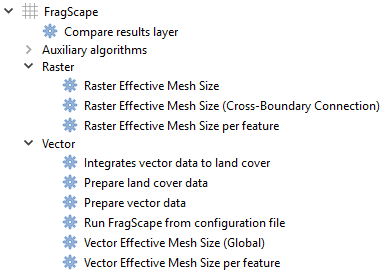
\includegraphics[scale=1]{pictures/algs_v2.png}
    \captionof{figure}{\tool Algorithms}
    \label{fig:algs}
\end{minipage}

\begin{enumerate}
    \item \texttt{Integrates vector data to land cover} : applies geometric difference/union between natural areas layer and additional data in vector mode
    \item \texttt{Prepare land cover data} : selection of natural areas from land cover layer in vector mode
    \item \texttt{Vector Effective Mesh Size (Global)} : computes fragmentation metrics in vector mode on the whole territory (features are dissolved if needed)
    \item \texttt{Vector Effective Mesh Size per feature} :  computes fragmentation metrics in vector mode for each feature of reporting layer
\end{enumerate}

\subsection{Results comparison}
\label{sec:cmp}

\tool\ finality is to study fragmentation evolution and so to compare results on a same territory at different times. Algorithm \texttt{Compare results layer} computes difference between 2 output layers of \tool\ on each field.

Difference on \texttt{effective\_mesh\_size} and \texttt{net\_product} fields is performed using CBC value if available.

Field \texttt{variation} contains effective mesh size evolution in percentage: $(B_{val} - A_{val} ) / (B_{val} + A_{val})$.

\subsection{Configuration file}

Configuration is saved as an XML file and thus can be opened in a text editor. Figure \ref{fig:configFile} shows the begining of configuration file \texttt{sample\_data/ECPI\_Clermontais\_2012/CBC/ECPI\_Clermontais\_2012\_CBC.xml}

\begin{figure}[h!]
    \centering
    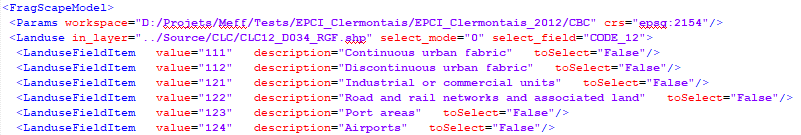
\includegraphics[scale=0.8]{pictures/configFile.png}
    \caption{Example of a configuration file}
    \label{fig:configFile}
    %\source{\tool\ v1.0}
\end{figure}

In \textit{Landuse} tag, one can see attributes such as \textit{in\_layer} (input layer), \textit{select\_mode} ($0$ meaning selection mode \texttt{By field values}) and \textit{select\_field} (selection field of input layer is \textit{CODE\_12}).
For each loaded field value, a \textit{LanduseFieldItem} tag exists and contains same attributes as in \tool\ (\textit{value}, \textit{description}, \textit{toSelect}).

Such file can be manually edited if needs be. For instance if relative paths must be changed for a new project (\texttt{../Source} becoming \texttt{../../Source}), updating it in \tool\ tables or creating a new project can be avoided by editing new paths in configuration file and then reloading it.

\section{FAQ}

\begin{itemize}
\item \textbf{Fields are not loaded in field/expression widget \includesvg{pictures/mIconExpression.svg}, why ?} If they don't appear, it is because associated layer is not loaded even if its path is displayed in combo box. Select another layer and then re-select initial layer.

\item \textbf{Which method should I use, CUT or CBC ?} CBC method has been designed to address boundary problem and then should be used. CUT method is available to allow comparison with already computed results, or in case boundaries are not a problem.

\item \textbf{Elements of fragmentation are already included in my land cover layer, should I run step 3 ?} In \tool\ 2.0, it is possible to specify step 4 input layer so taht step 3 is optional.

\item \textbf{Can I apply \tool\ processing to layer not produced by \tool\ ?} To apply \tool\ specific processing to specific data, one can use \tool\ algorithms described in section \ref{sec:algs}.

\end{itemize}

\frameboxbegin{Good practices}
\begin{itemize}
    \item Do not use spaces and special characters in file names.
    \item Do not use special characters in field values.
    \item Save \tool\ configuration at each step.
    \item Check each step result.
    \item If a problem occurs, save configuration, exit \tool\, relaunch \tool\ and re-open saved configuration. If problem still occurs, exit and relaunch QGIS. If problem still occurs, contact support team.
\end{itemize}
\frameboxend

\subsection{Error messages}
\label{sec:err}

\begin{itemize}
    \item \textbf{\color{red}Layer XXX is already loaded in QGIS, please remove it.} \tool\  cannot delete file if it is already loaded. Just remove it from QGIS project and relaunch \tool\ processing.
    \item \textbf{\color{red}The process cannot access the file because it is being used by another process: XXX.} Check that XXX file is not used by another process. If not, save configuration, save QGIS project, exit QGIS, relaunch QGIS, relaunch \tool, re-open configuration and relaunch \tool\ processing.
    \item \textbf{\color{red}Algorithm XXX not found} This error occurs if \tool\ installation failed. Try to uninstall and reinstall \tool. If error remains, please contact support team.
    %\item \textbf{\color{red}ModuleNotFoundError: No module named 'scipy'} Library \emph{scipy} is not installed. Install it and relaunch \qgis. On \emph{Linux}, install package \emph{python-scipy}. On \emph{Windows}, use \emph{OsGeo4W} installer.
    \item \textbf{\color{red}NameError: name 'np'|'scipy' is not defined}
    Library \emph{numpy}|\emph{scipy} is not installed. Install it and relaunch \qgis. On \emph{Linux}, install package \emph{python-numpy}|\emph{python-scipy}. On \emph{Windows}, use \emph{OsGeo4W} installer.
\end{itemize}

If an unknown error occurs, please report it at \url{https://github.com/MathieuChailloux/FragScape/issues}.

\textbf{\color{red}}



%\subsubsection*{}

\addcontentsline{toc}{section}{Bibliography}
\printbibliography

\end{document}